\documentclass[11pt]{article}
\usepackage[margin=1in]{geometry}
\usepackage{graphicx}
\usepackage{hyperref}
\usepackage{float}
\usepackage{booktabs}
\usepackage{xcolor}
\usepackage{enumitem}

\title{EDA: Canonical Dataset Restructure and Analysis}
\author{Pham Thanh Dat \\ \texttt{phamdat17092004@gmail.com}}
\date{May 2026}

\begin{document}
\maketitle

\section{Overview}

This report presents exploratory data analysis of the restructured canonical dataset
for the MycoAI fungal species project. The dataset has been reorganized into two
named source collections --- \texttt{curated\_primary} and
\texttt{incoming\_low\_quality} --- each with defined quality tiers and intended
uses. A unified preparation pipeline transforms raw source images into a canonical
derived hierarchy under \texttt{Dataset/prepared/}, organized by species, strain,
and environment.

The report covers: source collection profiles, species and environment
distributions, metadata quality assessment, the preparation pipeline architecture,
and the canonical hierarchy contract.

\section{Source Collections}

The dataset root now contains two named source collections:

\begin{itemize}[itemsep=4pt]
  \item \textbf{\texttt{curated\_primary}}: High-quality reference images with
    complete metadata (species, strain, environment, angle). Used for retrieval
    holdout evaluation, YOLO training, and fine-tuning.
  \item \textbf{\texttt{incoming\_low\_quality}}: Lower-quality images from
    diverse species with partial or missing metadata. Used for generalization
    testing and diverse data validation.
\end{itemize}

\begin{figure}[H]
\centering
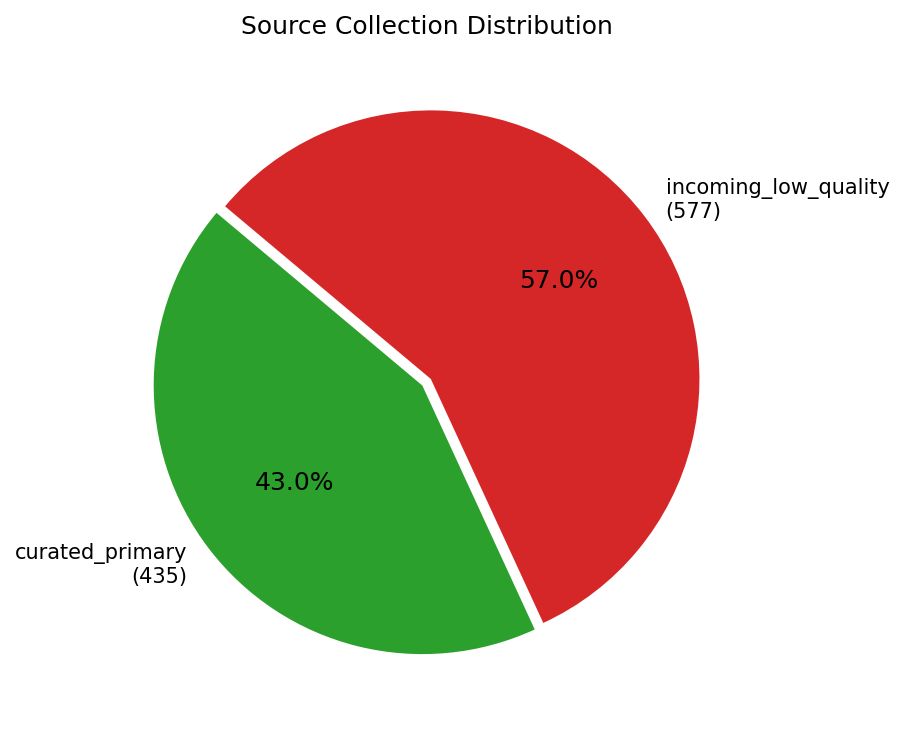
\includegraphics[width=0.55\textwidth]{images/collection_distribution.png}
\caption{Source collection distribution: \texttt{curated\_primary} (435) vs
\texttt{incoming\_low\_quality} (577)}
\label{fig:collection_distribution}
\end{figure}

\subsection{Collection Summary}

\begin{table}[H]
\centering
\begin{tabular}{lrr}
\toprule
\textbf{Metric} & \textbf{curated\_primary} & \textbf{incoming\_low\_quality} \\
\midrule
Images           & 435  & 577  \\
Species          & 8    & 65   \\
Strains          & 31   & 1*   \\
Environments     & 7    & 1*   \\
Parse success    & 100\% & 0\% \\
\bottomrule
\end{tabular}
\caption{Collection statistics. (*) Incoming metadata is unresolved ---
  all strains and environments fall back to \texttt{unknown}.}
\label{tab:collection_summary}
\end{table}

\section{Species Distribution}

\subsection{Curated Collection (8 species)}

The curated collection contains 8 \textit{Penicillium} species with 4--7 strains
per species (except \textit{P.~cyclopium} with 1 strain). This collection is the
primary source for strain holdout experiments in retrieval evaluation.

\begin{figure}[H]
\centering
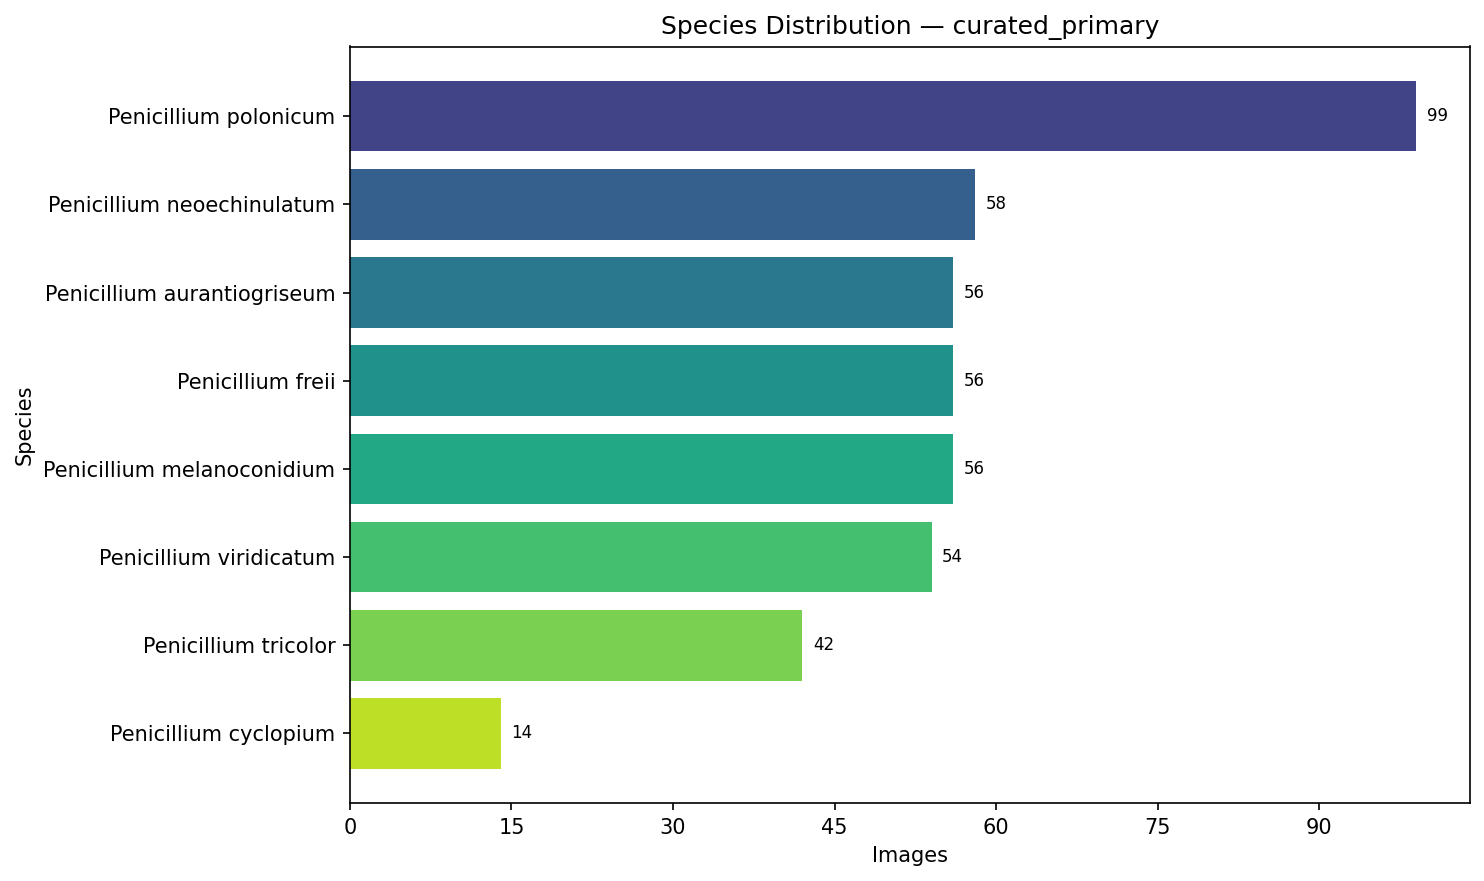
\includegraphics[width=0.85\textwidth]{images/curated_species.png}
\caption{Species distribution --- \texttt{curated\_primary}}
\label{fig:curated_species}
\end{figure}

\subsection{Incoming Collection (65 species)}

The incoming collection contains 65 fungal species, mostly from the
\textit{Aspergillus} and \textit{Penicillium} genera, with 1--2 strains per
species and 4--12 images per species.

\begin{figure}[H]
\centering
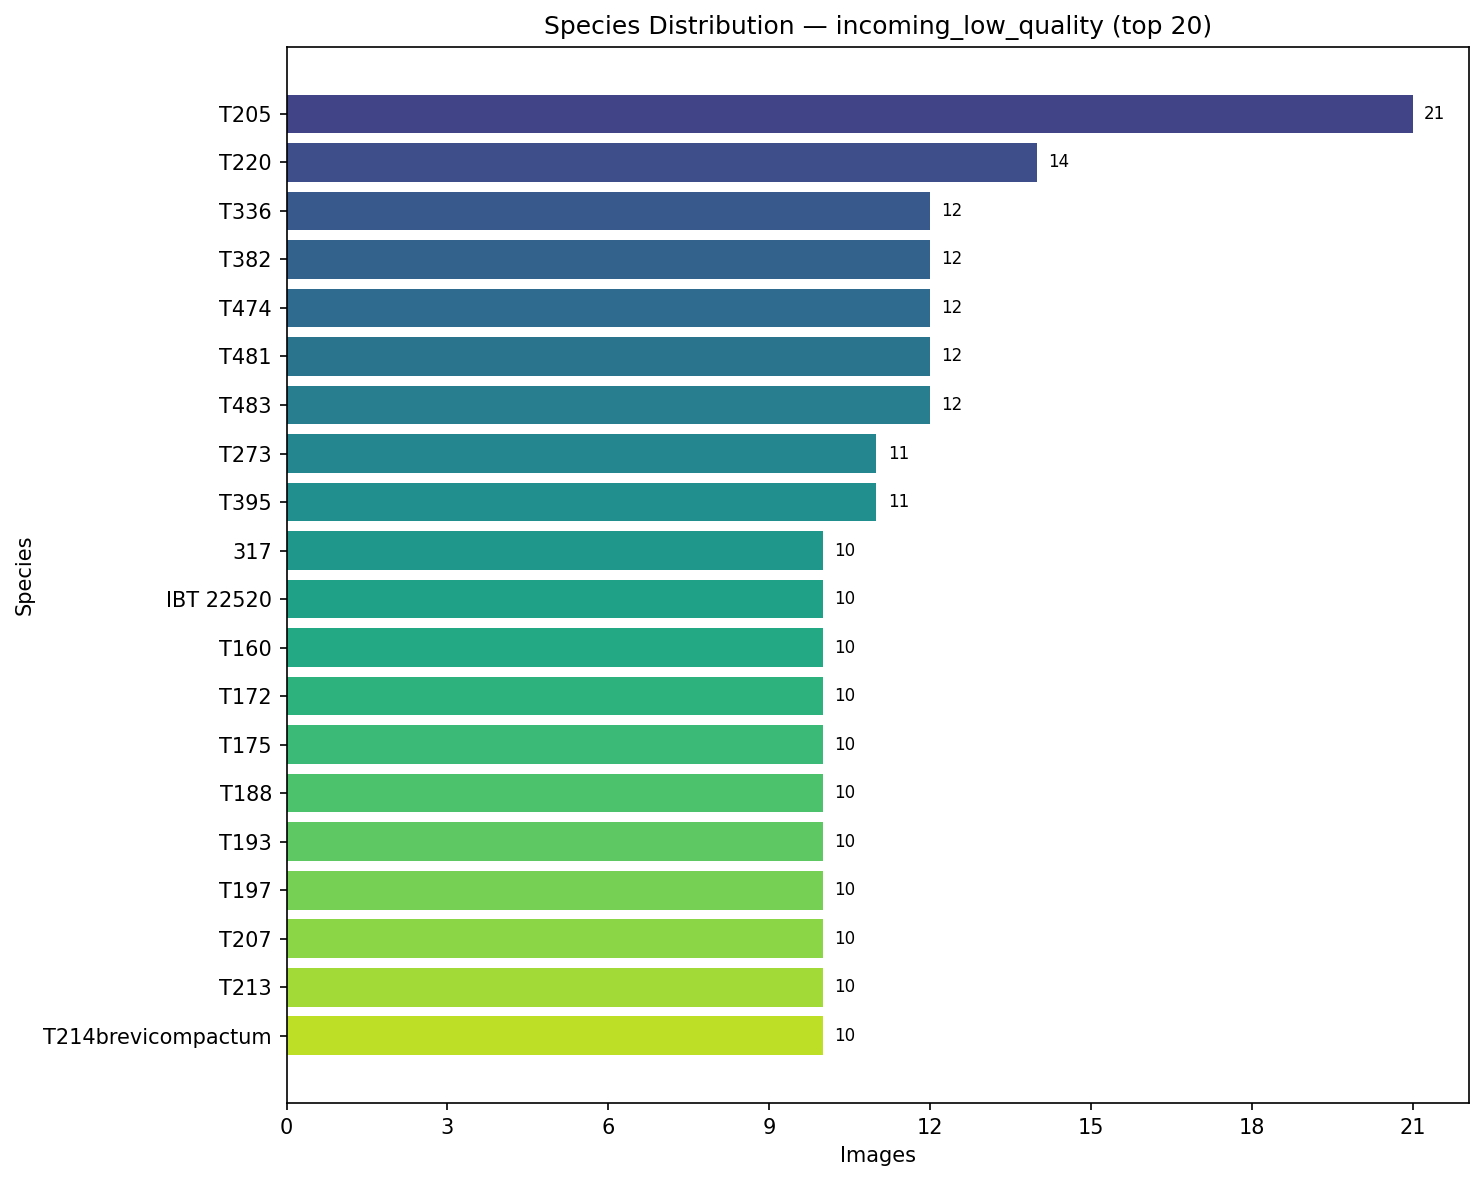
\includegraphics[width=0.9\textwidth]{images/incoming_species.png}
\caption{Species distribution --- \texttt{incoming\_low\_quality} (top 20)}
\label{fig:incoming_species}
\end{figure}

\section{Environment Distribution}

The curated collection spans 7 culture environments (CYA, MEA, YES, DG18, CREA,
CYA30, CYAS), each with 60--64 images --- well-suited for environment-invariant
feature learning. The incoming collection currently registers all 577 images as
\texttt{unknown} environment due to non-standard filename patterns.

\begin{figure}[H]
\centering
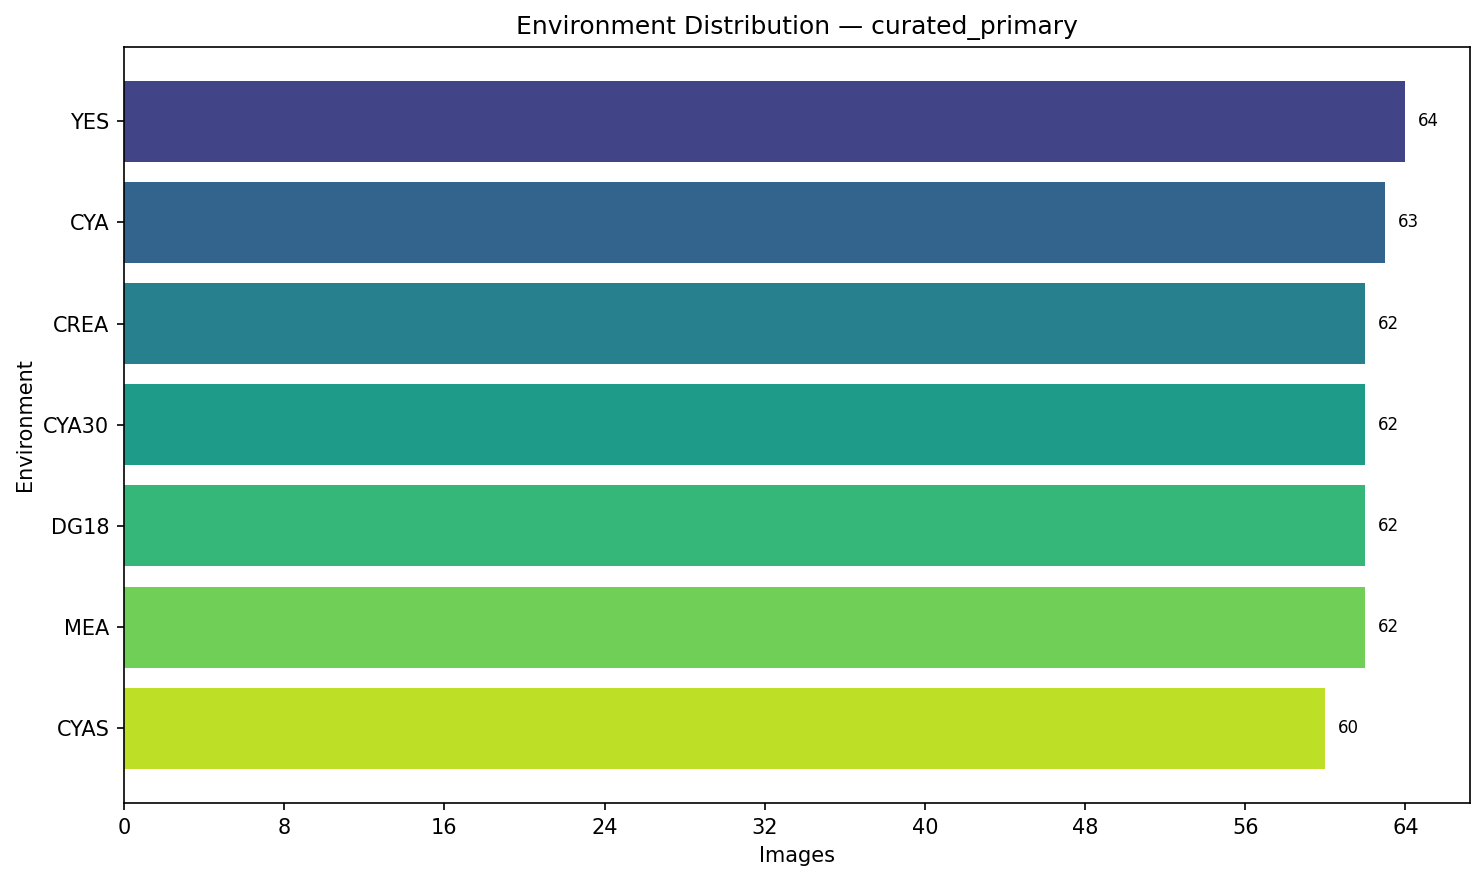
\includegraphics[width=0.8\textwidth]{images/curated_environments.png}
\caption{Environment distribution --- \texttt{curated\_primary}}
\label{fig:curated_environments}
\end{figure}

\section{Strain Distribution}

The curated collection contains 31 unique strains across 8 species. Most strains
have 14--16 images each, providing sufficient data for leave-one-strain-out
evaluation protocols.

\begin{figure}[H]
\centering
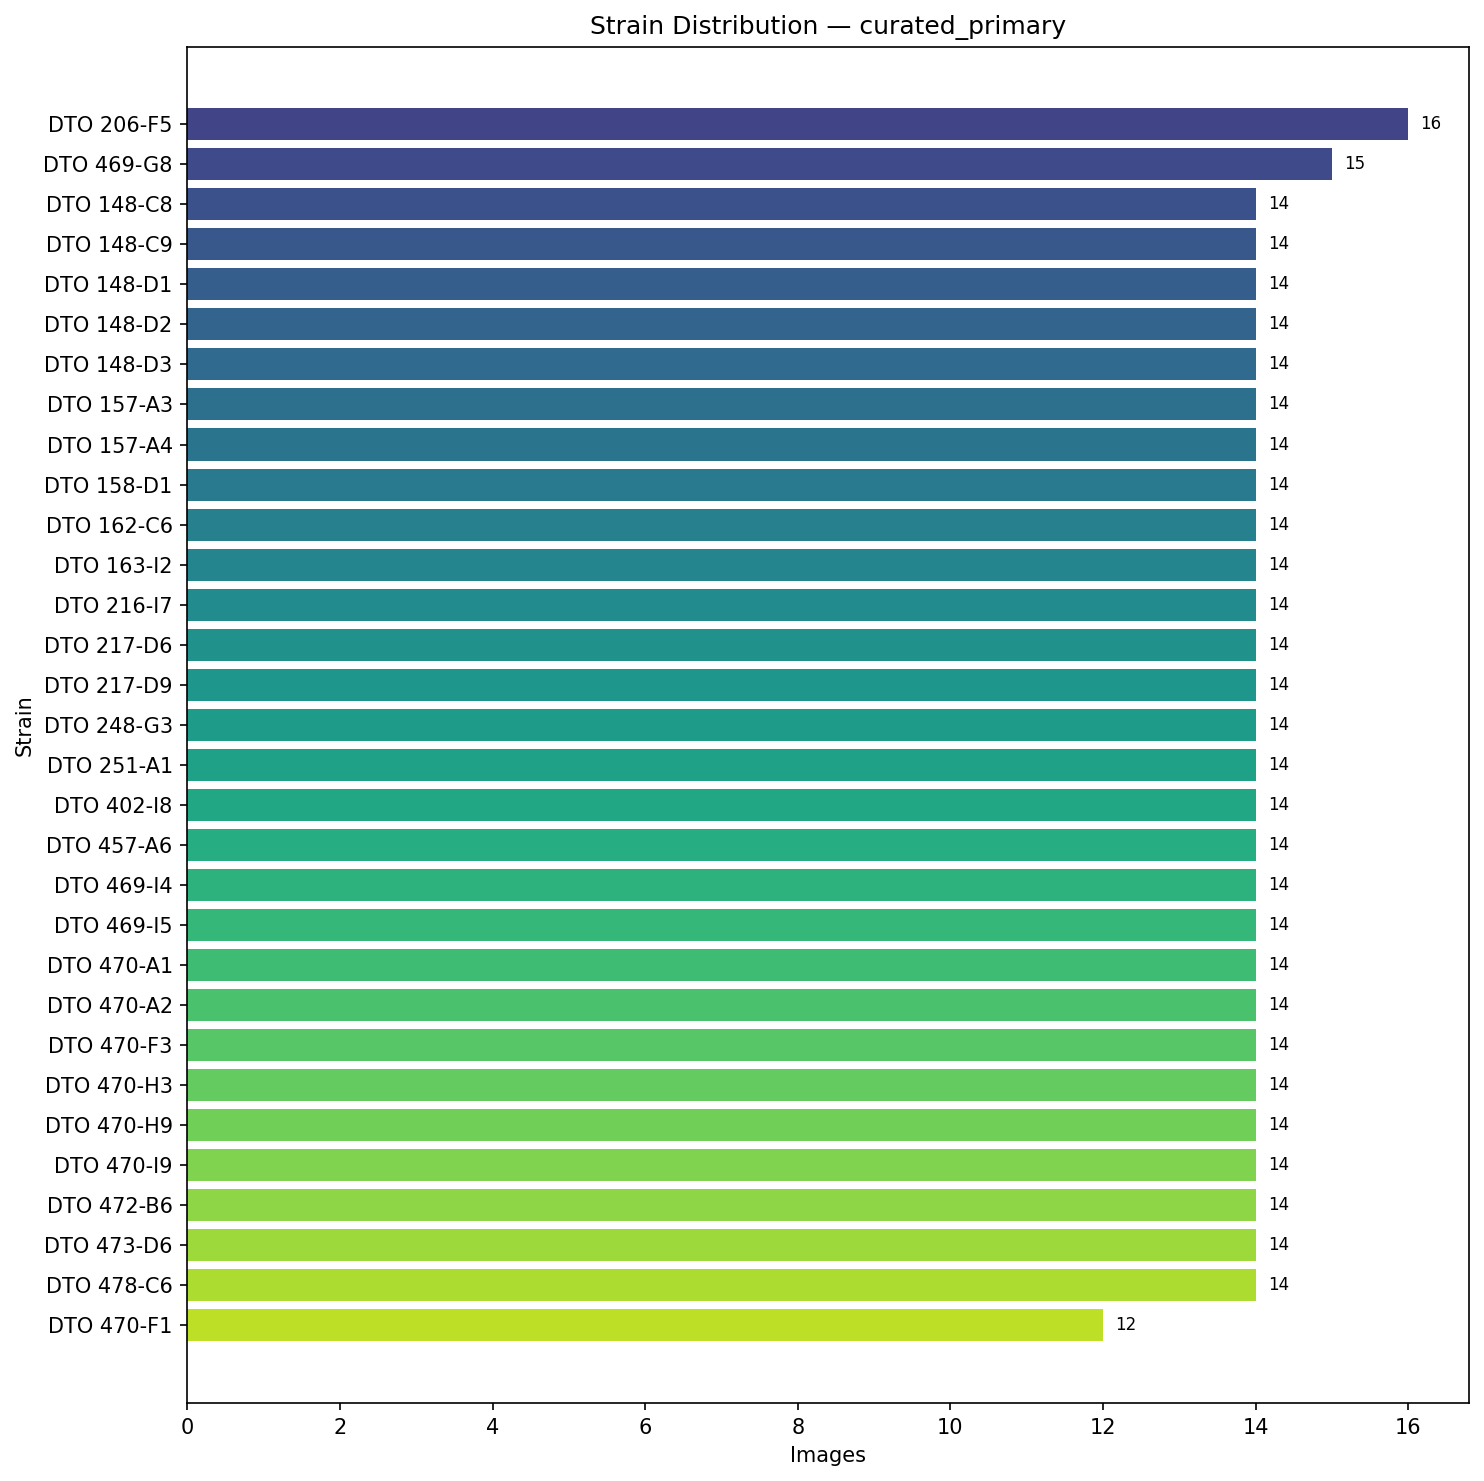
\includegraphics[width=0.9\textwidth]{images/curated_strains.png}
\caption{Strain distribution --- \texttt{curated\_primary}}
\label{fig:curated_strains}
\end{figure}

\section{Metadata Quality}

\begin{figure}[H]
\centering
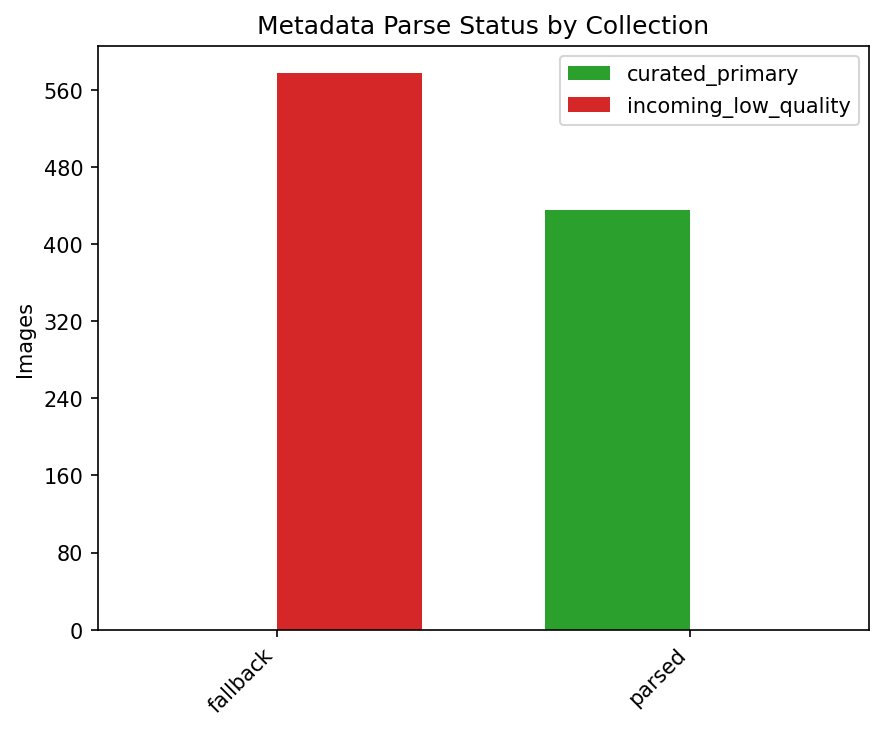
\includegraphics[width=0.65\textwidth]{images/parse_status.png}
\caption{Metadata parse status by collection}
\label{fig:parse_status}
\end{figure}

All 435 curated images parse successfully via structured filename patterns (e.g.,
\texttt{DTO~148-D1~MEAob}). All 577 incoming images fall through to folder-name-based
species inference due to non-standard naming. This is expected behavior given the
\texttt{incoming\_low\_quality} designation.

\section{Preparation Pipeline}

\begin{figure}[H]
\centering
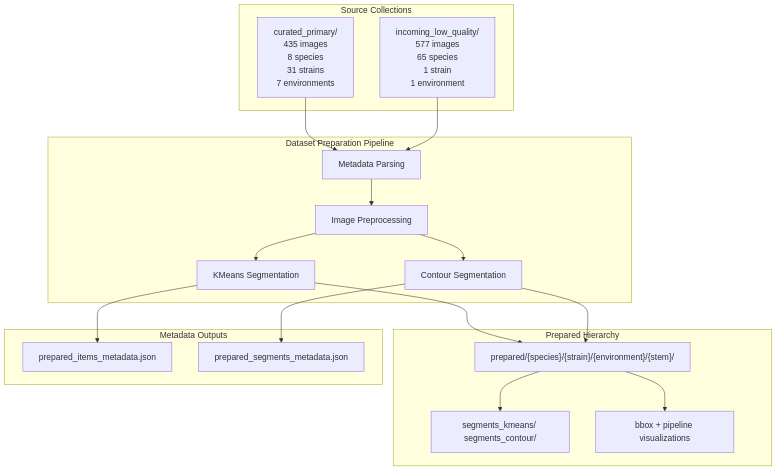
\includegraphics[width=0.95\textwidth]{images/dataset_pipeline.png}
\caption{Dataset preparation pipeline: source collections $\rightarrow$ metadata
$\rightarrow$ preprocessing $\rightarrow$ segmentation $\rightarrow$ prepared hierarchy}
\label{fig:pipeline}
\end{figure}

The unified preparation pipeline in \texttt{src/prepare/dataset.py} replaces the
legacy \texttt{reformat\_dataset.py} and \texttt{reformat\_dataset\_yolo.py}
scripts. Key features:

\begin{itemize}[itemsep=2pt]
  \item \textbf{Single entrypoint}: One script handles both source collections
  \item \textbf{Dual segmentation}: KMeans and contour-based methods for every image
  \item \textbf{Canonical output}: Organized as
    \texttt{prepared/\{species\}/\{strain\}/\{environment\}/\{stem\}/}
  \item \textbf{Path-authoritative metadata}: Consumers read
    \texttt{segment\_path} from JSON metadata instead of constructing flat paths
  \item \textbf{Visualization}: Bounding-box overlays and pipeline visualizations
    for both segmentation methods
\end{itemize}

\section{Canonical Hierarchy Contract}

\begin{table}[H]
\centering
\begin{tabular}{ll}
\toprule
\textbf{Path Component} & \textbf{Description} \\
\midrule
\texttt{source.jpg}     & Original source image copy \\
\texttt{prepared.jpg}   & Preprocessed (resized, normalized) image \\
\texttt{item.json}      & Per-image metadata record \\
\texttt{segments\_kmeans/}  & KMeans segmentation output (3 segments) \\
\texttt{segments\_contour/} & Contour segmentation output (3 segments) \\
\texttt{bbox\_*.jpg}    & Bounding-box overlay visualization \\
\texttt{pipeline\_*.jpg} & Full pipeline visualization \\
\bottomrule
\end{tabular}
\caption{Canonical prepared item directory contents}
\label{tab:canonical_layout}
\end{table}

\section{Key Findings}

\begin{enumerate}[itemsep=3pt]
  \item \textbf{Total dataset}: 1,012 images across 73 species, 32 strains, and 8 environments
  \item \textbf{Curated collection} (435 images) is metadata-rich and suitable for
    controlled evaluation; all 7 environments are well-represented
  \item \textbf{Incoming collection} (577 images) brings species diversity (65
    species) but requires metadata enrichment before it can support
    environment-aware experiments
  \item \textbf{Strain imbalance}: \textit{Penicillium cyclopium} has only 1 strain
    (14 images) vs 4--7 strains for other curated species --- this is a known
    limitation for retrieval holdout protocols
  \item \textbf{Canonical hierarchy} is operational: \texttt{prepared/} output
    follows \texttt{\{species\}/\{strain\}/\{environment\}/\{stem\}/} structure
  \item \textbf{Legacy fallback}: \texttt{Dataset/original/} and
    \texttt{Dataset/new\_data/} still work when canonical
    \texttt{curated\_primary/} and \texttt{incoming\_low\_quality/} paths are absent
\end{enumerate}

\section{Environment Configuration}

Dataset paths are configurable via environment variables:

\begin{table}[H]
\centering
\begin{tabular}{lll}
\toprule
\textbf{Variable} & \textbf{Default} & \textbf{Description} \\
\midrule
\texttt{MYCOAI\_ROOT}   & Auto-detected       & Monorepo/workspace root \\
\texttt{DATASET\_ROOT}  & \texttt{\$MYCOAI\_ROOT/Dataset} & Shared dataset folder \\
\texttt{WEIGHTS\_DIR}   & \texttt{\$MYCOAI\_ROOT/weights}  & Model checkpoints \\
\texttt{RESULTS\_DIR}   & \texttt{\$MYCOAI\_ROOT/results}  & Experiment outputs \\
\bottomrule
\end{tabular}
\caption{Configurable path environment variables}
\label{tab:env_vars}
\end{table}

Set \texttt{DATASET\_ROOT} to an external path (e.g., SSD mount, Vast.ai volume)
while preserving the canonical folder structure.

\section{Conclusion}

The dataset restructure from flat legacy paths to a canonical
\texttt{curated\_primary} / \texttt{incoming\_low\_quality} / \texttt{prepared}
hierarchy establishes clear provenance, quality tiering, and predictable
downstream consumption patterns. The unified preparation pipeline eliminates
code duplication between the old \texttt{reformat\_dataset.py} and
\texttt{reformat\_dataset\_yolo.py} scripts while adding contour segmentation
as a second method alongside KMeans. All downstream code paths (feature
extraction, Qdrant upload, retrieval evaluation) have been updated to consume
metadata-provided \texttt{segment\_path} fields rather than constructing flat
paths from \texttt{Dataset/segmented\_image/}.

\end{document}
